\documentclass[a4paper]{ctexart}
%\usepackage{fdsymbol}
\usepackage{graphicx}
\usepackage{epstopdf}
\usepackage{mathtools,amsmath,amsthm,amsfonts,bm}
\usepackage{booktabs}
\usepackage{xcolor}
\usepackage{multirow}
\usepackage{threeparttable}
\usepackage{listings}
\usepackage{cases}
\usepackage{fancyhdr}


\usepackage[left=1in,right=1in,top=0.8in,bottom=1in]{geometry}%设置页边距

\title{\vspace{-0.3in}\textbf{Advanced Econometrics}}
\author{\textbf{姓名:宋其来 \quad 学号:502024740012}\\(Due Monday, October 28 in class)}
\date{}

\theoremstyle{remark}
\newtheorem*{solution}{解}
\renewcommand{\qedsymbol}{证毕}

\pagenumbering{arabic}
\pagestyle{plain}
\begin{document}
\maketitle
\textbf{Important: }
The empirical exercises should be done in Stata and a copy of your Stata code should be turned in along with your homework. Your homework should be typed/handwritten (you will grab results from the computer output and edit them), it should not contain irrelevant material (when you edit strip out things that are not useful), and it should be a clear and neat presentation of the results (insert comments where necessary in your codes).
%%第一小问
\begin{itemize}
    %%第一小问
    \item [\textbf{1.}]The data in the file Koop-Tobias.csv are used in Koop and Tobias’s (2004) study of the relationship between wages and education, ability, and family characteristics. Their data set is a panel of 2,178 individuals with a total of 17,919 observations. The variables are defined in the article. Let $X_{1}$ equal a constant, education, experience, and ability (the individual’s own characteristics). Let $X_{2}$ contain the mother’s education, the father’s education, broken home, and the number of siblings (the household characteristics). Let $Y$ be the log of the hourly wage.
    \begin{enumerate}
        \item[i.]Compute the least squares regression coefficients in the regression of $Y$ on $X_{1}$ . Report the coefficients in a table (same for the following regressions)
        \item[ii.]Let’s verify the Frish-Waugh-Lowell Theorem. Regress each of the three variables in $X_{2}$ (excluding Broken home) on all the variables in $X_{1}$ and save the residuals into a matrix $X_{2}^{*}$ . Then regress y on $X_{1}$ and $X_{2}^{*}$ . How do your results compare to the results of the regression of y on $X_{1}$ and $X_{2}$ (excluding Broken home)?
        \item[iii.]Run the regression of $y$ on $X_{1}$ and $X_{2}$ . Test for the presence of heteroscedasticity using both White’s general test and the Breusch-Pagan (1980) and Godfrey (1988) Lagrange multiplier test. Do your results suggest the presence of the heteroscedasticity? Report the result along with the correct SE. How do the results change from part i? Based on your results, what is the estimate of the marginal value, in \$/hour, of an additional year of education, for someone who has 12 years of education when all other variables are at their means and $Broken home=0$ ?
        \item[iv.]Use an F testv. Use an F statistic to test the joint hypothesis that the coefficients on the four household variables in $X_{2}$ are zero.
        \item[vi.]We are interested in possible nonlinearities in the effect of education on log wage. (Koop and Tobias focused on experience. As before, we are not attempting to replicate their results.) Plot a histogram of the education variable, which will show values from 9 to 20, a spike at 12 years (high school graduation), and a second at 15.Consider aggregating the education variable into a set of dummy variables:
        \begin{center} 
            $HS=1\ if \ Educ \leq 12,0 \  otherwise$\\
            $Col=1  \ if \ Educ>12 \ and \ Educ \leq 16,0 \  otherwise$\\
            $Grad = 1 \  if \ Educ>16,0 \  otherwise.$
        \end{center}
            Replace Educ in the model with (Col, Grad), making high school (HS) the base category, and recompute the model. Report all results. How do the results change? Based on your results, what is the marginal value of a college degree? What is the marginal impact on log wage of a graduate degree?
        \item[vii.] The aggregation in part vi actually loses quite a bit of information. Another way to introduce nonlinearity in education is through the function itself. Add Educ2 to the regresssion in part iii and recompute the model. Again, report all results. What changes are suggested? Test the hypothesis that the quadratic term in the equation is not needed - that is, that its coefficient is zero.
        \item[viii.]One might suspect that the value of education is enhanced by greater ability. We could examine this effect by introducing an interaction of the two variables in the equation. Add the variable $\\ Educ_Ability = Educ \times Ability$ to the base model in part iii. Now, what is the marginal value of an additional year of education?
    \end{enumerate}

%%第一题解
    \begin{solution}
        i.在回归之前首先对变量进行线性检验。所得的散点图如下:\\
        \begin{figure}[h]
            \centering
            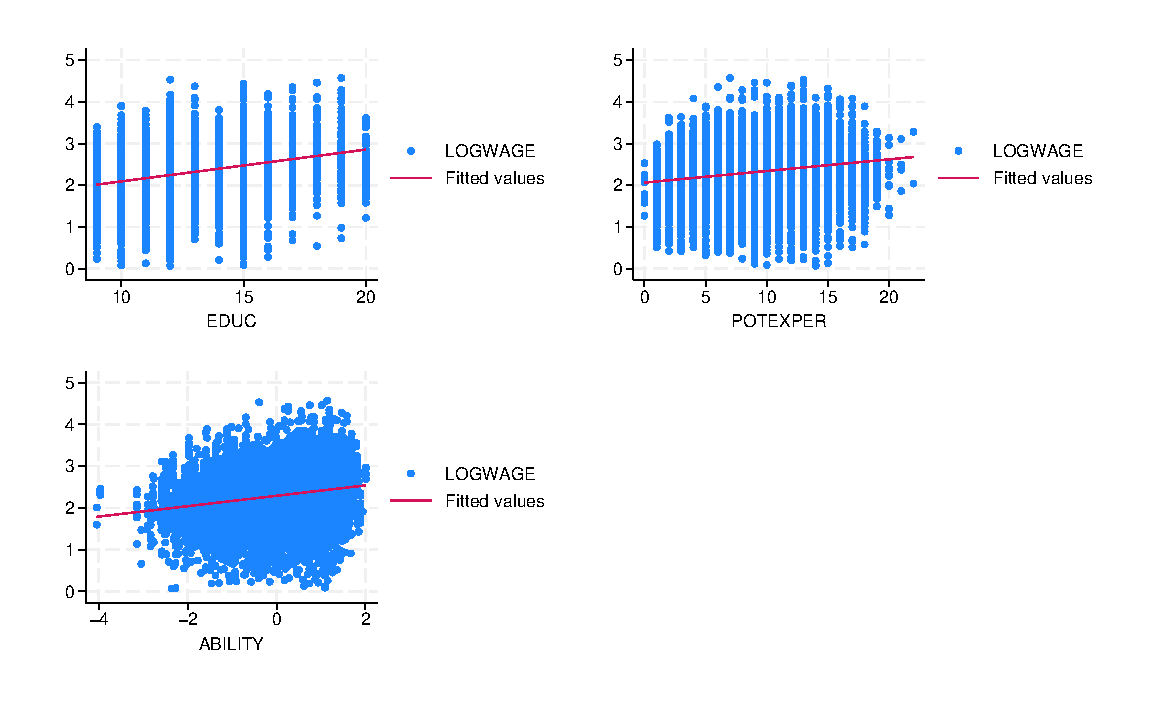
\includegraphics[scale=0.8]{hw2i.eps}
            \caption{$x_1$的散点图}
        \end{figure}
        由图可知,$x_i$的三个变量基本符合线性假设。进行回归并且进行共线性检验得到的结果如下:
        \clearpage  
        \begin{table}[h]
            \centering
            \begin{tabular}{llll}%%l表示左对齐,c表示居中对齐,r表示右对齐,p表示百分数
                \hline
                variables & coefficient & P-value\\
                \hline
                educ &  0.0737621  & 0.00\\
                potexpri & 0.0394896  & 0.00\\
                ability & 0.0828907 & 0.00 \\
                constant & 1.027229 & 0.00\\
                VIF & \multicolumn{2}{c}{1.30}\\
                \hline
            \end{tabular} 
            \caption{\label{font-table} regression results \& VIF} 
        \end{table}
        由上表可知,回归满足多重共线性假设,不存在多重共线性。系数如上。\\
        ii. 根据题目要求,对于$X_2$中的三个变量,分别进行回归并且保存残差。然后对$Y$进行回归,其中残差系数和变量系数如下表2所示:
        \begin{table}[h]
            \centering
            \begin{tabular}{lll|lll}%%l表示左对齐,c表示居中对齐,r表示右对齐,p表示百分数
                \hline
                variables & coefficient & P-value & variables & coefficient & P-value\\
                \hline
                educ &  0.0722035  & 0.00 & educ &  0.0737621  & 0.00\\
                potexpri & 0.0395093  & 0.00 & potexpri &  0.0394896  & 0.00\\
                ability & 0.0774678 & 0.00 & ability &  0.0828907  & 0.00\\
                \hline
                mothered & -0.000117  & 0.00 & resid\_mother &  -0.000117  & 0.945\\
                fathered & 0.0054569  & 0.00 & resid\_father &  0.0054569  & 0.00\\
                siblings & 0.0047656 & 0.00 & resid\_siblings &  0.0047656  & 0.00\\
                constant & 0.9695096 & 0.00 & constant &  1.027229  & 0.00\\
                \hline
            \end{tabular} 
            \caption{\label{font-table} regression residuals} 
        \end{table}\\
        由上表知,带有残差作为回归元的残差系数与对应变量的系数相同,同时其他变量的系数也基本相同。残差系数不变的原因是由于$X_1$和$X_2$的变量之间线性相关,即$X_2$可以被$X_1$的变量表示,那么原来的$X_2$系数即表示其独特的那部分,因此残差也是表示与其他变量无关的部分,同时其他的变量的系数产生编变化。\\

        iii.由题意知,对于$Y$,$X_1$和$X_2$进行回归,结果如下:
        \begin{table}[h]
            \centering
            \begin{tabular}{lll}%%l表示左对齐,c表示居中对齐,r表示右对齐,p表示百分数
                \hline
                variables & coefficient & P-value \\
                \hline
                educ &  0.0711887  & 0.00 \\
                potexpri & 0.0395104  & 0.00 \\
                ability & 0.0773688 & 0.00 \\
                mothered & 0.000071  & 0.967 \\
                fathered & 0.0053168  & 0.00 \\
                siblings & 0.0048714 & 0.007  \\
                brknhome & -0.0528695 & 0.00  \\
                constant & 0.9896543 & 0.00  \\
                \hline
            \end{tabular} 
            \caption{\label{font-table} regression in general} 
        \end{table}\\
        同时进行White检验和BP检验来验证异方差性,结果如下:
        \begin{table}[h]
            \centering
            \begin{tabular}{llll}%%l表示左对齐,c表示居中对齐,r表示右对齐,p表示百分数
                \hline
                 & White test & BP test & GL test\\
                \hline
                $\chi^2$ &  190.48  & 139.05 & 3469.021\\
                p-value & 0.00 & 0.00 & 0.00 \\
                \hline
            \end{tabular} 
            \caption{\label{font-table} White test\& BP test\&GL test} 
        \end{table}\\
        以上两个检验的原假设都是存在同方差,由表3知,三个检验的p值都小于0.05,因此拒绝原假设,即认为存在异方差。\\
        因此进行异方差稳健的标准误d的回归,与标准误差对比结果如下:\\
        \begin{table}[h]
            \centering
            \begin{tabular}{lll}%%l表示左对齐,c表示居中对齐,r表示右对齐,p表示百分数
                \hline
                variables & std err & robust err \\
                \hline
                educ &  0.0022572  & 0.0023585 \\
                potexpri & 0.0008986  & 0.0009037 \\
                ability & 0.0049336 & 0.0049804 \\
                mothered & 0.0016954  & 0.001715 \\
                fathered & 0.0013379  & 0.0013548 \\
                siblings & 0.0017912 & 0.0017806  \\
                brknhome & 0.0099904 & 0.0101058  \\
                constant & 0.0338945 & 0.0335674  \\
                \hline
            \end{tabular} 
            \caption{\label{font-table} regression in general} 
        \end{table}\\
        由表5可以看出,稳健标准误与非稳健标准误相比,基本没有变化。\\
        且经过计算其额外一年教育的边际价值(以美元 / 小时为单位)的估计值是2.304955 。\\








        \qedsymbol
    \end{solution}




    \clearpage  
    %第二题
    \item [\textbf{2.}]Critical Summary Writing. Pick a published paper from top journals (AER, Econometrica, JPE, QJE, RES, JF, JFE, RFS, JFQA, MS) that uses field/quasi experiments for causal inference. The paper should be different from those in the presentation list. Write a summary of the paper in your own words in no more than 500 words (in English). Do not copy and paste the abstract of the paper. Pay particular attention to the experimental design, empirical methodology, and how the authors address internal and external validity concerns.
    
    %%第二题解
    \begin{solution}
        




        \qedsymbol
    \end{solution}

    %%排除块
    \iffalse
    \fi


\end{itemize}
\end{document}